\section{Results}

\subsection{What mineral and dietary data exists in the LSDA, and can it be obtained}

Harvesting the complete LSDA experiment catalog returned \LSDATotal{} records,
of which \LSDAHuman{} concern human subjects. \LSDARelevant{} mention a mineral
or a nutritional topic, and \LSDAMeasured{} list a mineral or nutritional
variable among the parameters actually measured --- the stricter and more useful
criterion. Calcium is the most frequently measured (\LsdameasCa{} experiments),
followed by phosphorus (\LsdameasP), iron (\LsdameasFe), sodium (\LsdameasNa)
and potassium (\LsdameasK). Boron, a plant micronutrient rather than a human
clinical analyte, was measured in \LsdameasB{} experiments, as expected for an
archive dominated by human and animal physiology.

Accessibility is the limiting factor. Of the \LSDAMeasured{} experiments that
measured a mineral or nutritional variable, only \LsdaaccessOpen{} are openly
available, \LsdaaccessRequestrequired{} require a formal data request,
\LsdaaccessNotsubmitted{} were never submitted to the archive, and
\LsdaaccessHeldelsewhere{} are held by another repository
(Figure~\ref{fig:lsda}). Restricting to human studies measuring three or more
minerals leaves 57 experiments, of which 9 are open and 40 request-gated.

\begin{figure}[htbp]
  \centering
  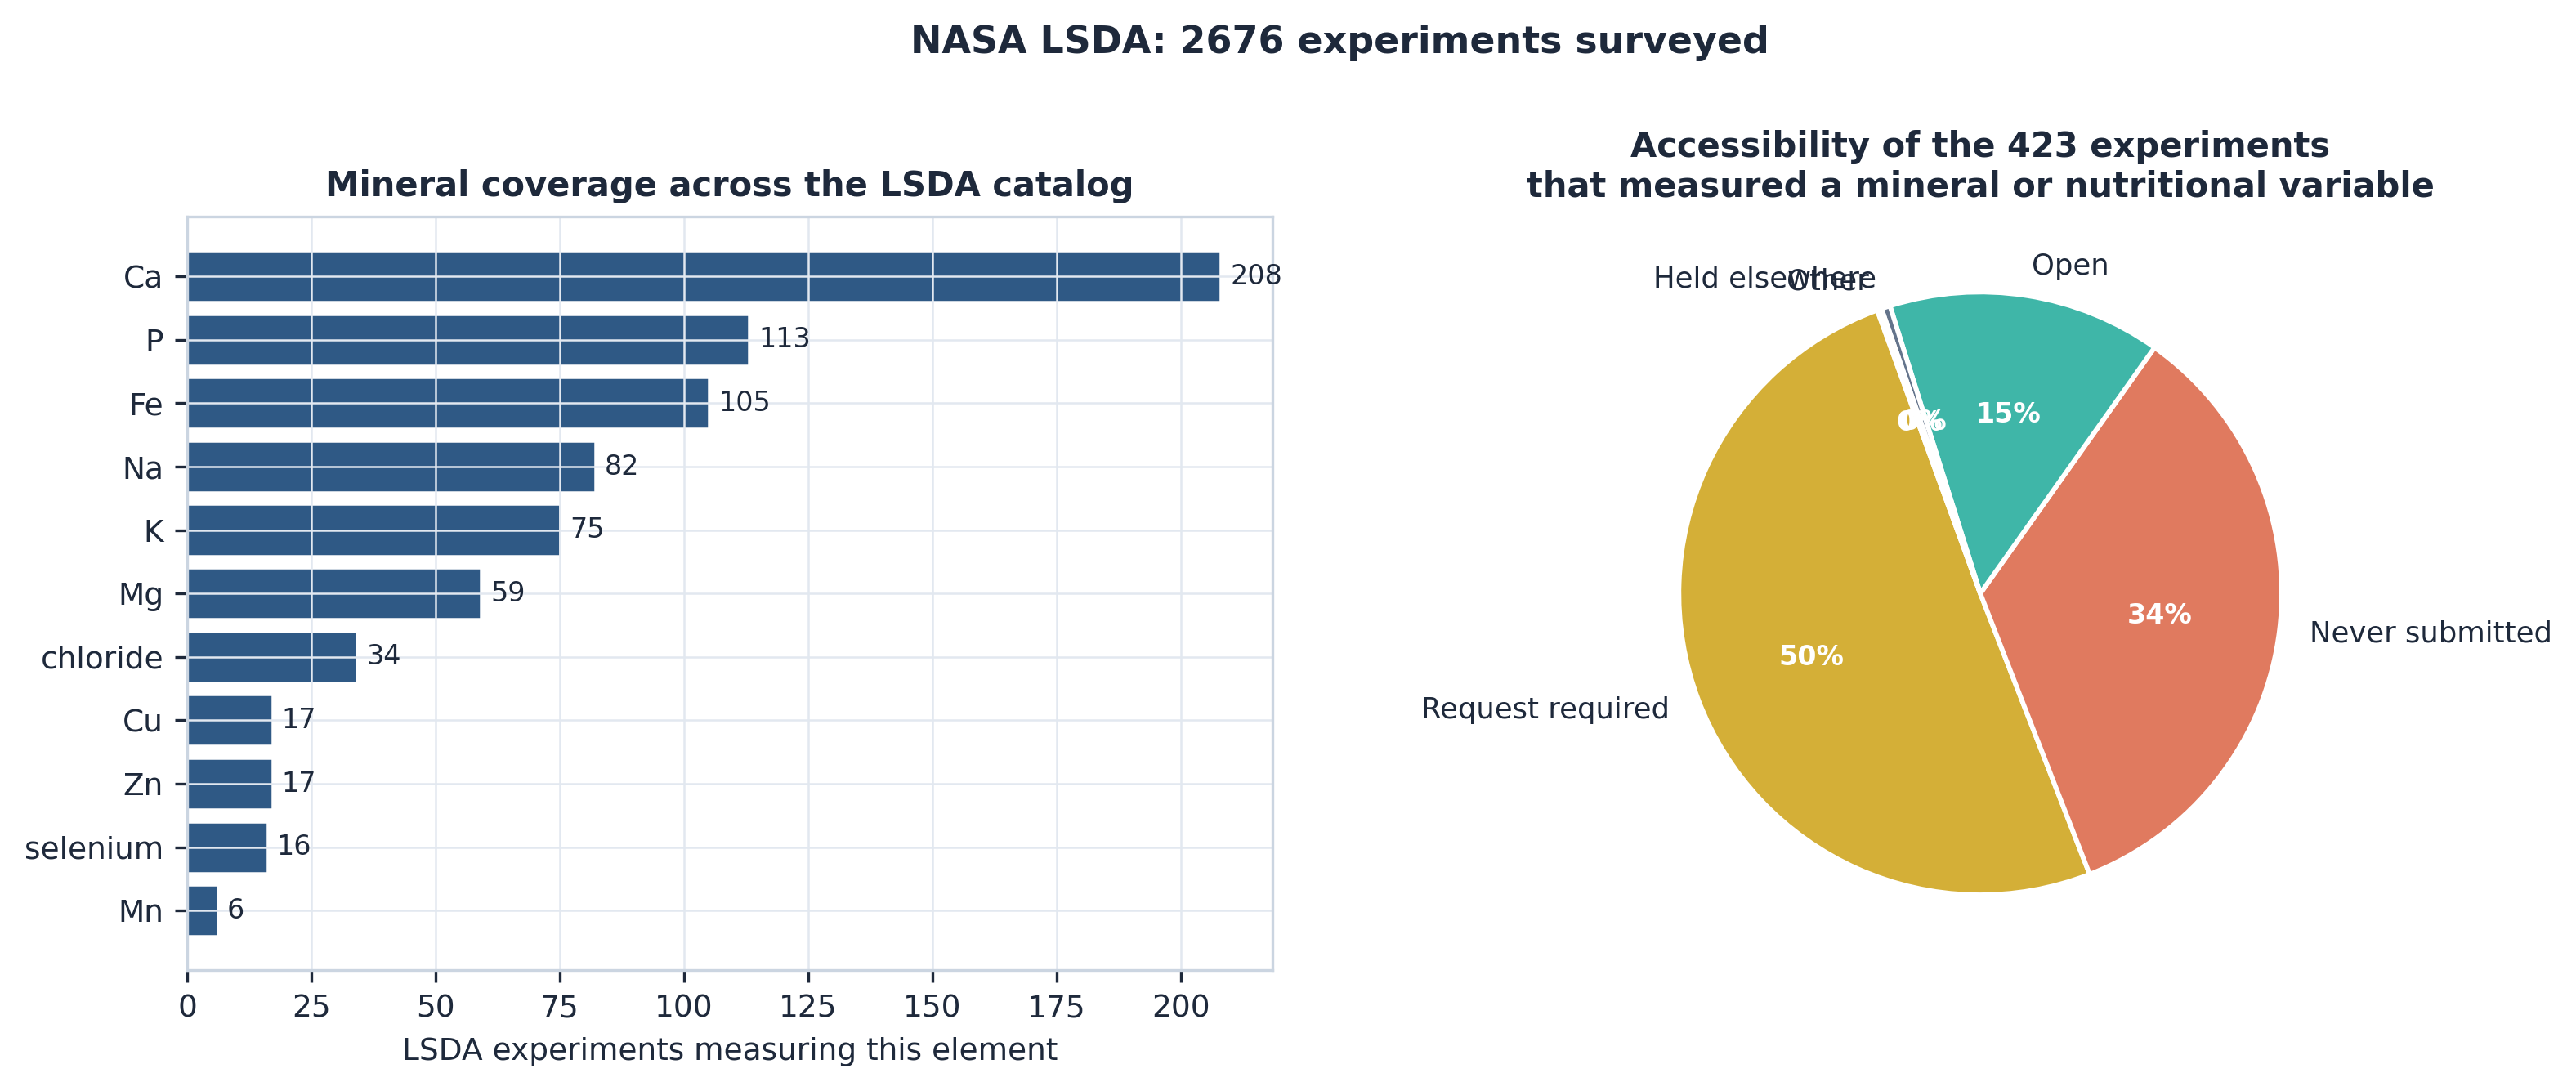
\includegraphics[width=\textwidth]{figures/fig7_lsda_landscape.png}
  \caption{Mineral and dietary data across the NASA Life Sciences Data Archive.
    Left: number of experiments measuring each element. Right: accessibility of
    the \LSDAMeasured{} experiments that measured a mineral or nutritional
    variable. Access, not measurement, is the binding constraint.}
  \label{fig:lsda}
\end{figure}

The survey identifies the Nutritional Status Assessment (SMO-016E) as the
highest-value target for this question: it measured ten minerals across
long-duration ISS missions with in-flight sampling, and underlies the
time-resolved analysis of \citet{zheng2023}. It is request-gated. Also
surfaced were the NASA Biochemical Profile Project, Food Physiology, and
Clinical Nutritional Assessment (MR016G), the last of which is openly
available.

\subsection{A unit-labelling defect inverts the cross-study comparison}

The OSD-655 elemental file and its archived data dictionary both label calcium,
potassium, magnesium, phosphorus and sulfur as mg/g dry weight. Taken at face
value, mean potassium is $2943\%$ of dry weight, magnesium $805\%$, calcium
$651\%$, sulfur $551\%$ and phosphorus $367\%$ --- each impossible.
Reinterpreted as $\mu$g/g, all five fall within the normal range for leafy
\emph{Brassica} tissue and agree with the independently-scaled OSD-745 lettuce
values. The six elements OSD-655 already labels in $\mu$g/g require no change
and agree across studies without correction, which localises the defect
precisely. \NUnitOverrides{} column corrections were applied, and all four
quality-control gates then passed.

The consequence is not cosmetic. Concatenating the two studies without this
correction places five of twelve elements on a scale 1000-fold larger in one
crop than the other, which would dominate any distance-based method, any
principal component analysis, and any model trained on the pooled data.

\subsection{The two crops diverge in their flight response}

At face value the two studies look very different. In lettuce, flight/ground
concentration ratios sit close to unity across the board --- calcium
\FcLetCa{}, potassium \FcLetK{}, iron \FcLetFe{} --- and no element reaches
significance. In Tokyo Bekana, eight elements rise together: sodium
\FcTbNa{}, sulfur \FcTbS{}, potassium \FcTbK{}, iron \FcTbFe{}, phosphorus
\FcTbP{}, boron \FcTbB{}, calcium \FcTbCa{} and magnesium \FcTbMg{}, with
\NSigConc{} significant at $q<0.05$.

A coordinated rise of that kind is the signature of a dry-matter dilution
effect rather than eight independent uptake changes, and the centred log-ratio
analysis separates the two (Figure~\ref{fig:clr}).

\begin{figure}[htbp]
  \centering
  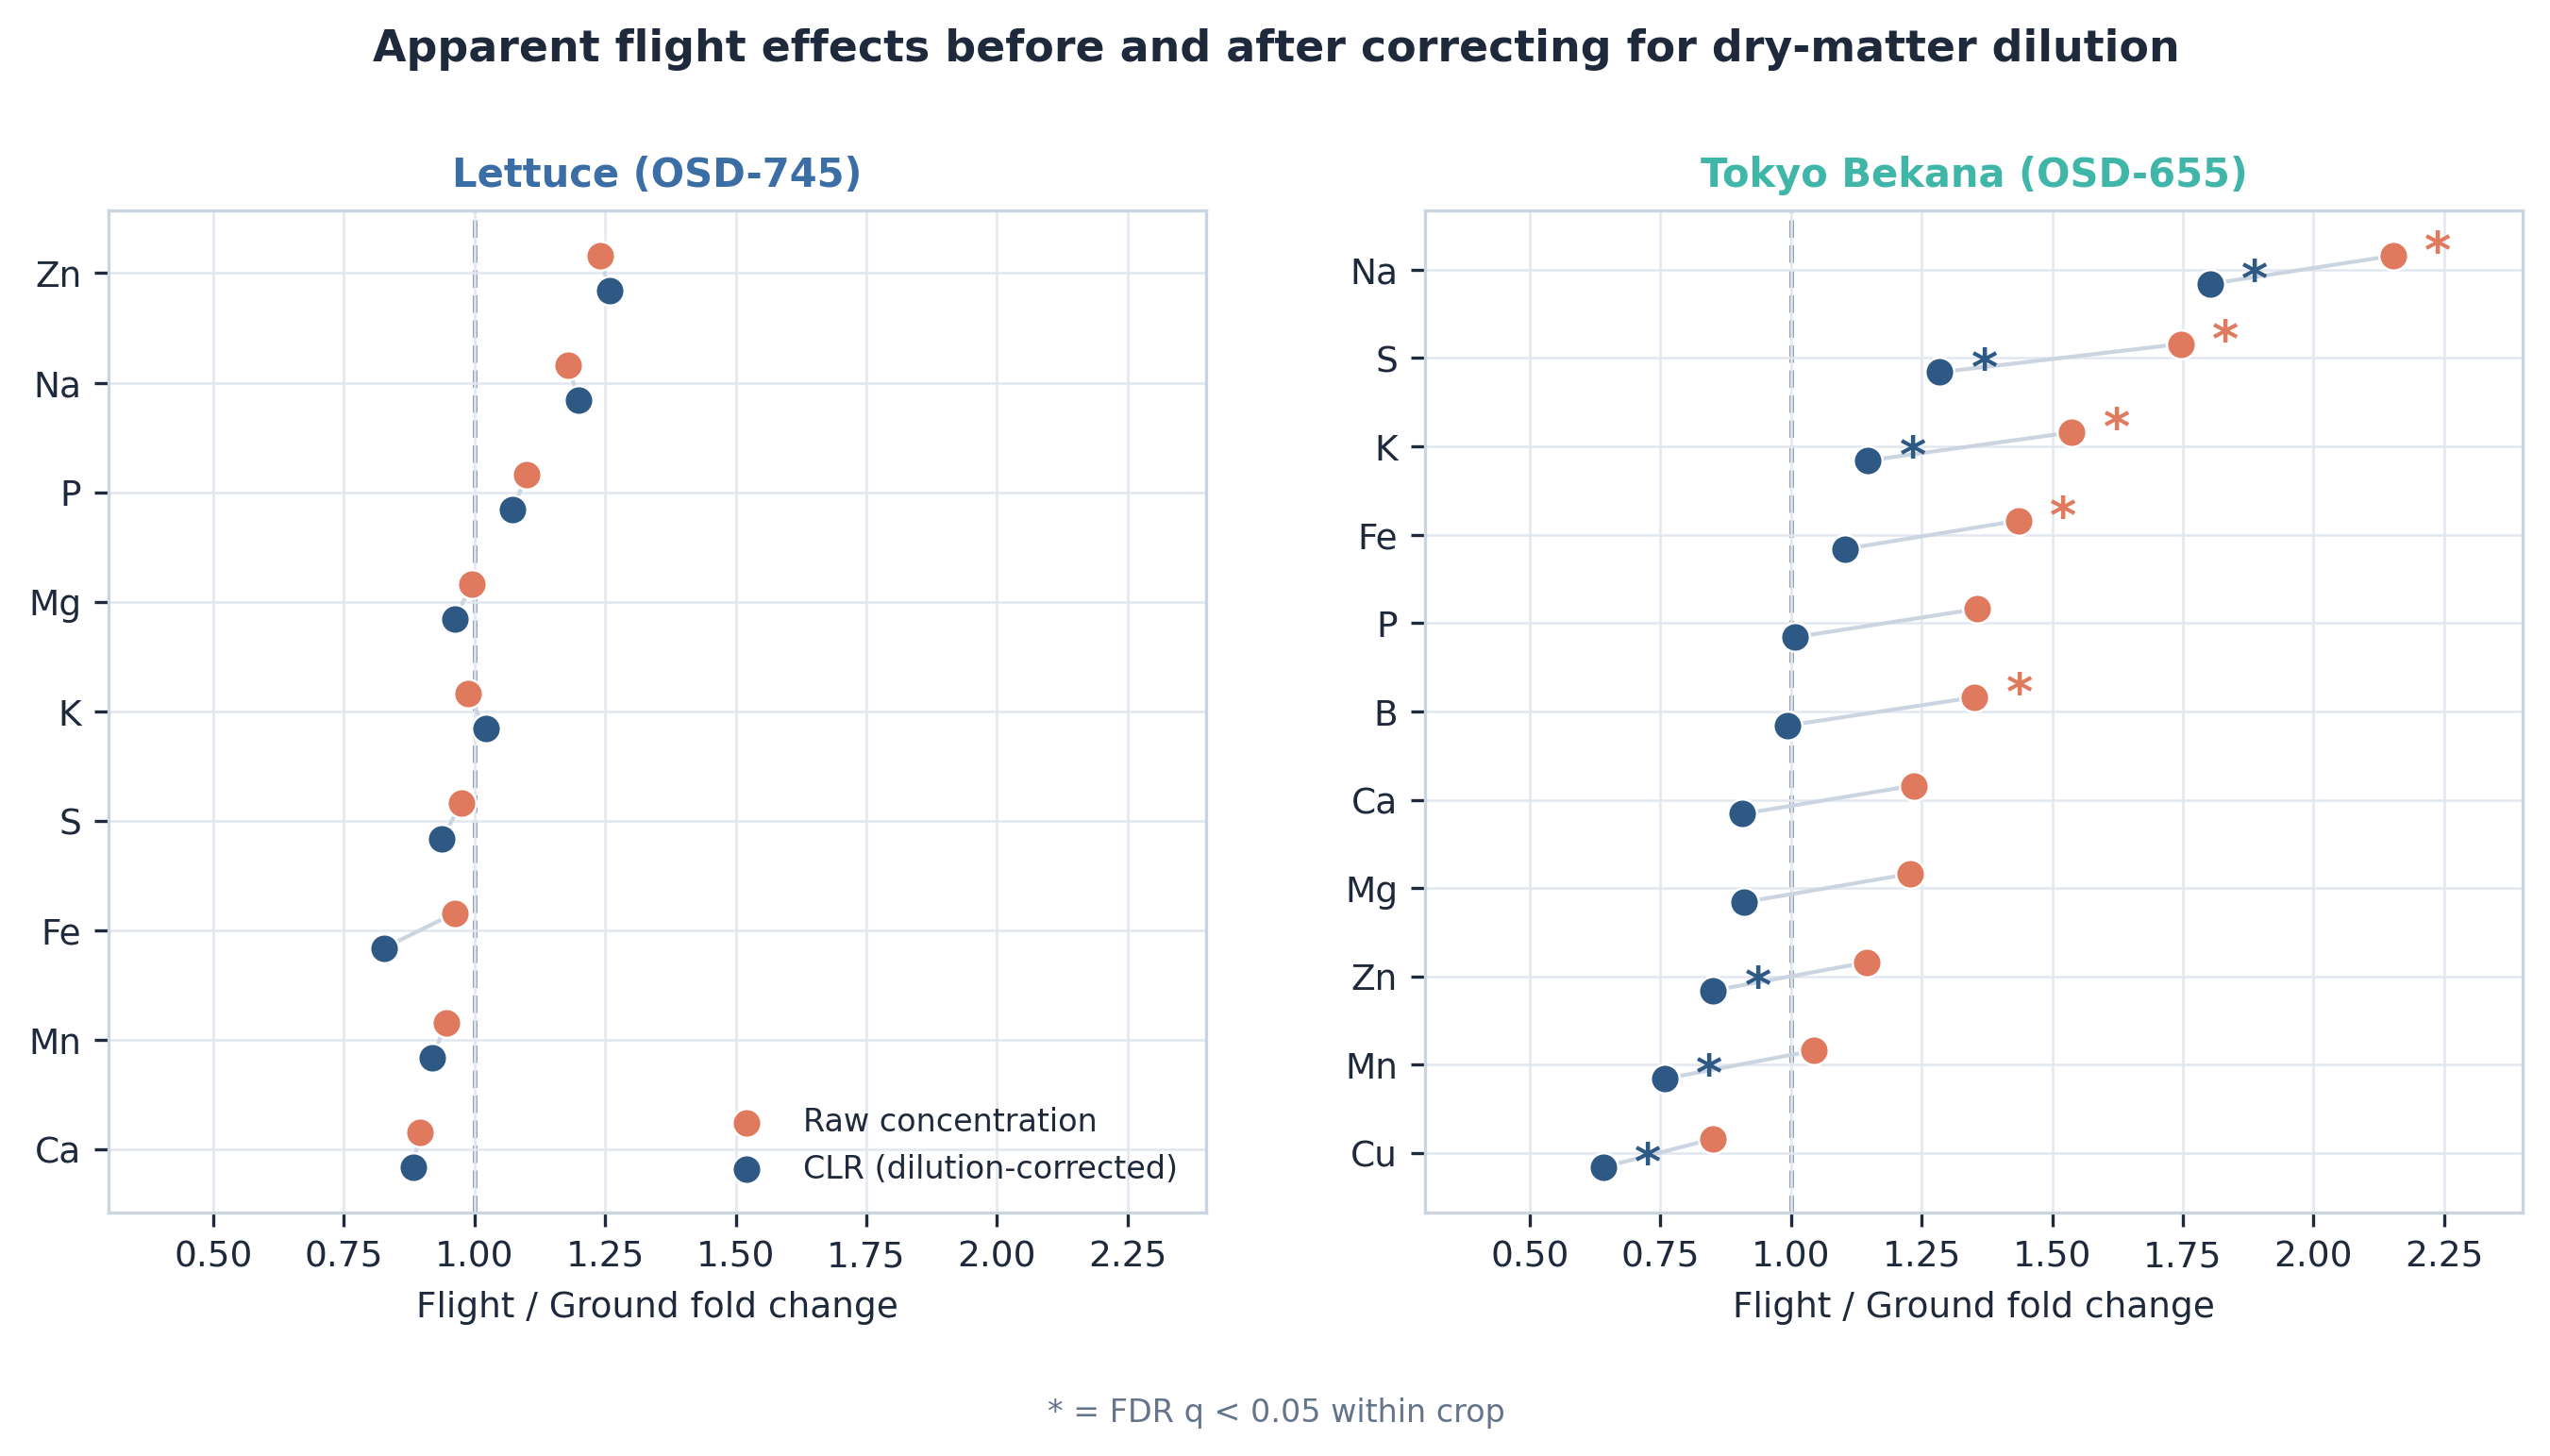
\includegraphics[width=\textwidth]{figures/fig1_fold_change_clr.png}
  \caption{Flight/ground fold changes before (coral) and after (navy)
    correcting for dry-matter dilution by centred log-ratio transform.
    Lettuce shows no significant change on either scale. In Tokyo Bekana the
    apparent calcium, magnesium, iron, boron and phosphorus increases collapse
    toward unity after correction, while sodium, sulfur and potassium persist.
    Asterisks mark $q<0.05$ within crop.}
  \label{fig:clr}
\end{figure}

After correction, \NSigCLR{} elements remain significant in Tokyo Bekana and
none in lettuce. Critically for the accumulation hypothesis that motivated this
work, the two divalent cations do not survive: calcium falls from \FcTbCa{} to
\FcclrTbCa{} ($q=\QclrTbCa$) and iron from \FcTbFe{} to \FcclrTbFe{}
($q=\QclrTbFe$). Both apparent increases are dilution artefacts. Potassium
persists (\FcTbK{} to \FcclrTbK{}, $q=\QclrTbK$), as do sodium (\FcclrTbNa)
and sulfur (\FcclrTbS). Copper, manganese and zinc become significantly
\emph{lower} in flight tissue once the composition is accounted for.

Only \NSigBoth{} elements --- potassium, sodium and sulfur --- are significant
on both scales, and these are monovalent cations and an anion, not the divalent
cations of the original hypothesis. Comparing the crops element by element
(Figure~\ref{fig:divergence}), \NDivergentCLR{} elements move in opposite
directions after correction (\DivergentElementsCLR).

\begin{figure}[htbp]
  \centering
  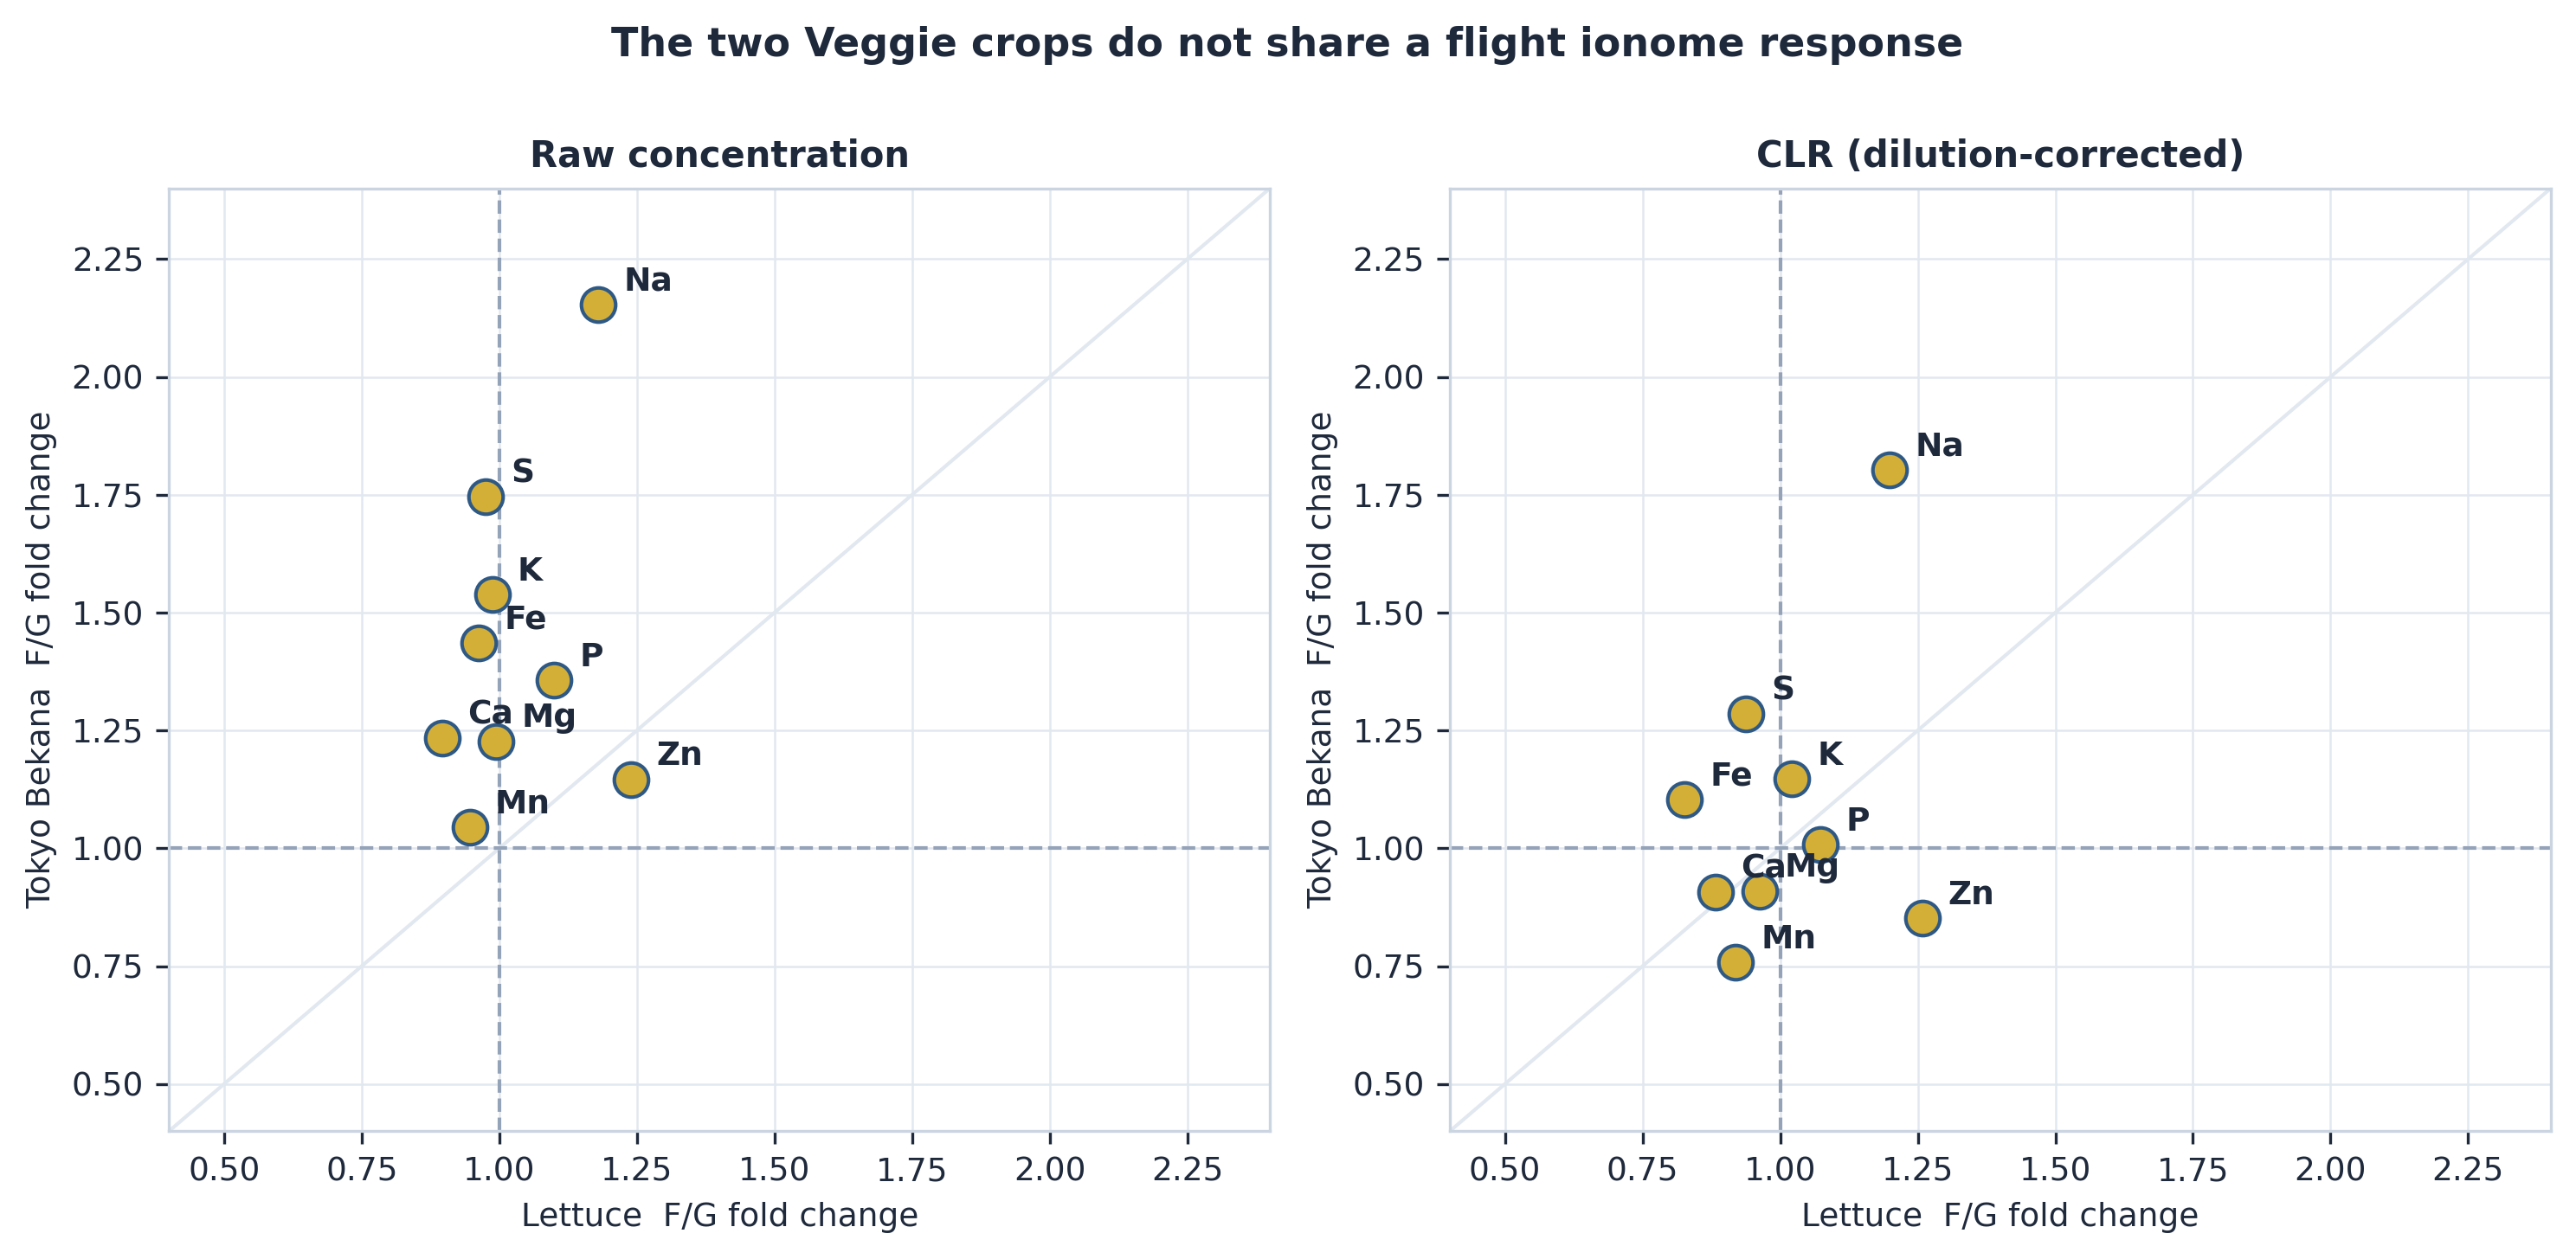
\includegraphics[width=\textwidth]{figures/fig2_crop_divergence.png}
  \caption{Lettuce versus Tokyo Bekana flight/ground fold change per element.
    Points on the diagonal would indicate a shared response. They do not lie on
    it on either scale.}
  \label{fig:divergence}
\end{figure}

\subsection{No flight signature transfers between crops}

Classification of flight versus ground from the ionome
(Figure~\ref{fig:ml}) confirms this from the opposite direction. Under
leave-one-mission-out cross-validation (\MlfoldsMission{} folds) the random
forest reaches \MlMissionRf{} balanced accuracy against a best baseline of
\MlbaselineMission{}, a margin of \MlMissionRfMargin{} with a 95\% confidence
interval of \MlMissionRfCi{} that spans chance. Penalised logistic regression
performs worse than baseline (\MlMissionLrMargin).

Under leave-one-crop-out --- training on one species and testing on the other
--- both models fall \emph{below} baseline (\MlCropRfMargin{} and
\MlCropLrMargin). A model that has learned the flight signature of one crop is
worse than useless on the other. That is not a failure of the method; it is a
direct measurement of the divergence, and it stands against previously reported
cross-species accuracies for this data that were not derived from any
implemented cross-species split.

\begin{figure}[htbp]
  \centering
  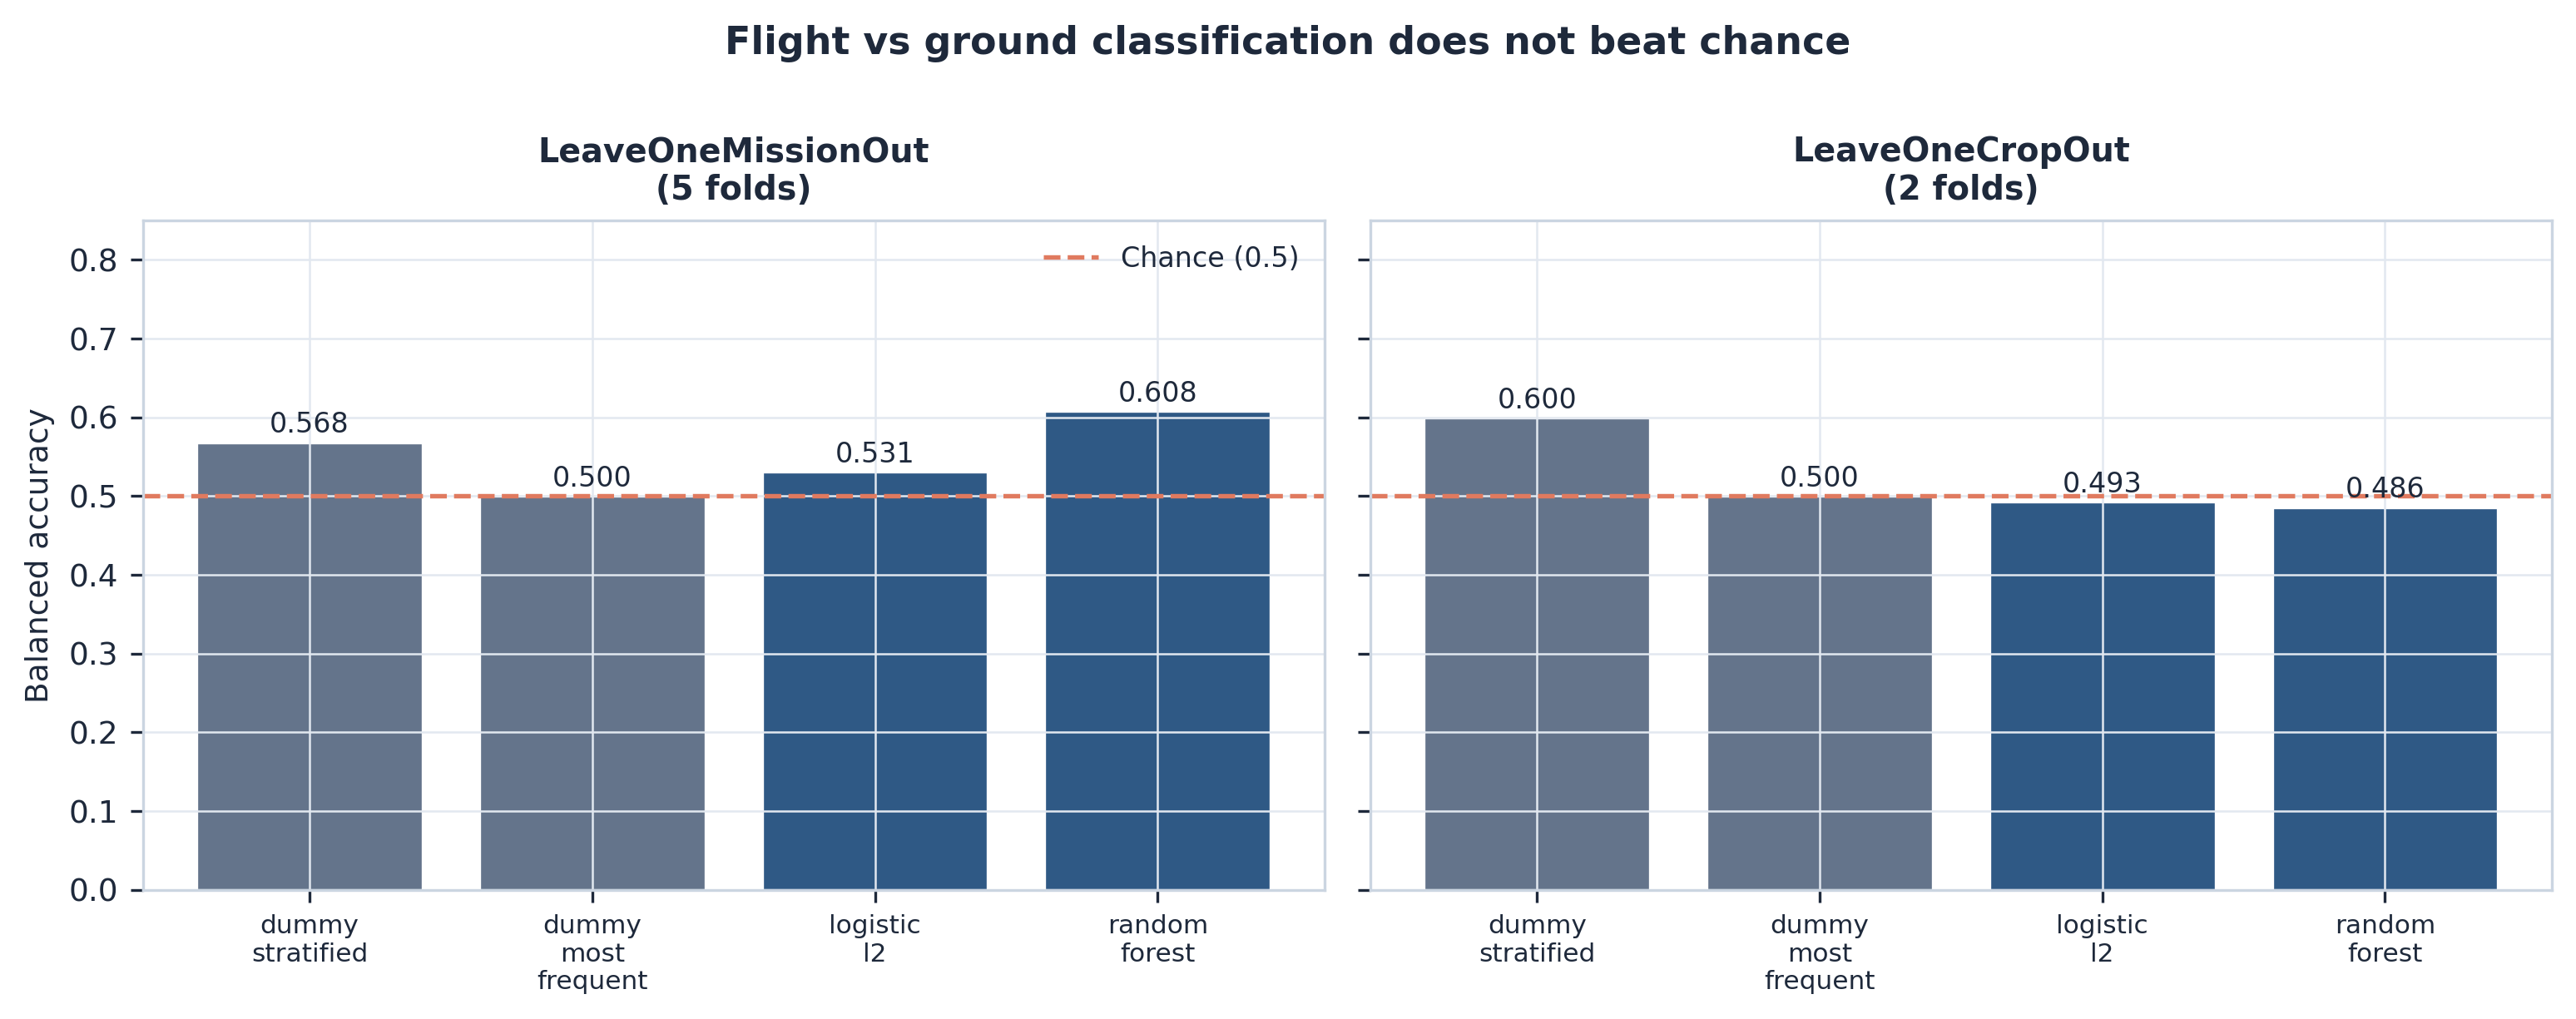
\includegraphics[width=0.92\textwidth]{figures/fig6_ml_performance.png}
  \caption{Balanced accuracy under both grouped cross-validation schemes,
    with the dummy baselines each model must beat.}
  \label{fig:ml}
\end{figure}

Permutation importance ranks \MltopOne, \MltopTwo{} and \MltopThree{} highest,
matching the three elements that survive compositional correction --- an
internal consistency between two methods that share no machinery.

\subsection{Astronaut serum minerals}

The Inspiration4 comprehensive metabolic panel provides \AstroObs{}
observations across \AstroN{} crew and \AstroTimepoints{} timepoints
(Figure~\ref{fig:serum}). Relative to each subject's pre-flight mean, potassium
fell in \AstrodownK{} of \AstroN{} crew at first return (median
\AstropctK\%), calcium in \AstrodownCa{} of \AstroN{} (median \AstropctCa\%),
and bicarbonate in \AstrodownCarbondioxide{} of \AstroN{}.

\begin{smacaution}[title=These data cannot establish a spaceflight effect]
Four subjects, a \AstroDuration-day mission, and no in-flight sample --- every
timepoint is pre-flight or post-return. The direction of change is reported
descriptively, per subject; no inferential test is appropriate at this size, and
none is performed.
\end{smacaution}

\begin{figure}[htbp]
  \centering
  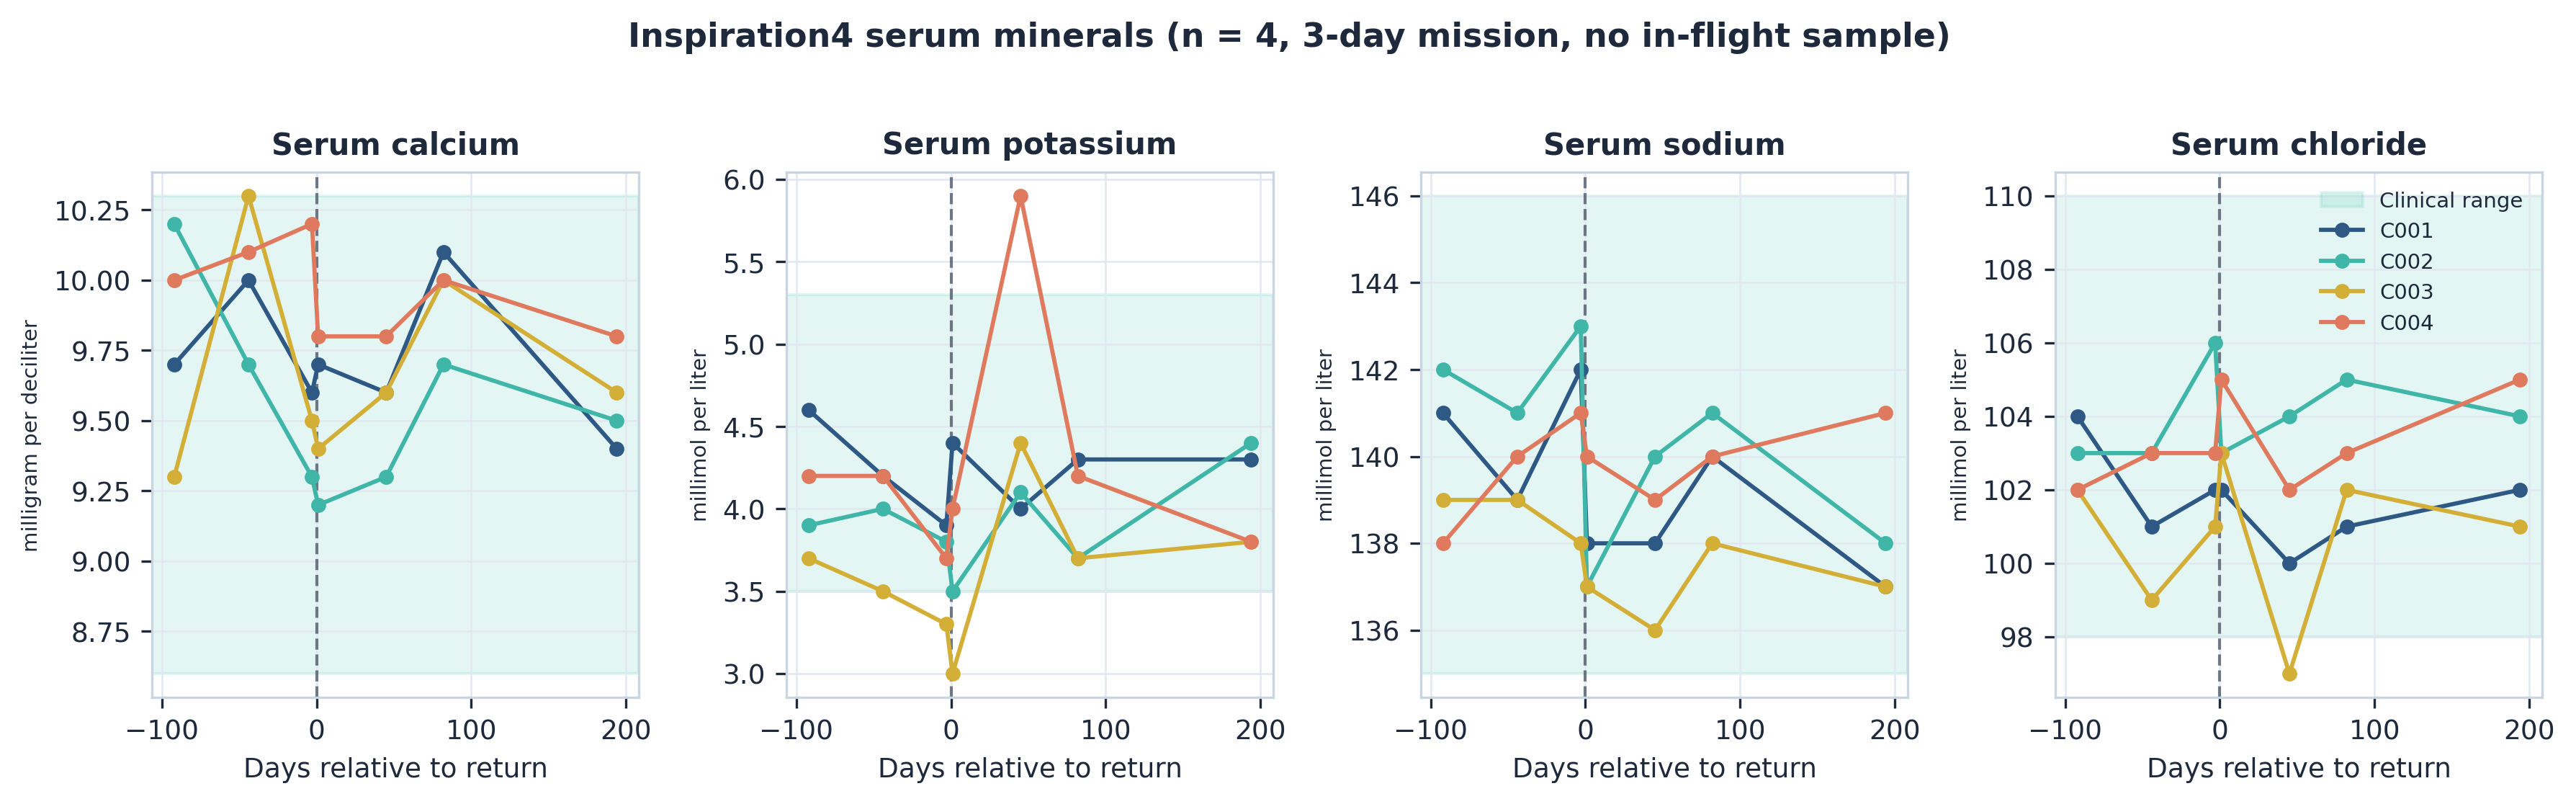
\includegraphics[width=\textwidth]{figures/fig4_astronaut_serum.png}
  \caption{Per-subject serum mineral trajectories, with the clinical reference
    range shaded. The dashed line marks return.}
  \label{fig:serum}
\end{figure}

\subsection{What a serving delivers, and whether overload is achievable}

Combining measured tissue concentrations with NASA daily requirements
\citep{jsc67378} gives the contribution of a realistic serving
(Figure~\ref{fig:serving}). A 100\,g fresh serving of flight-grown tissue at
$10\%$ dry matter supplies \ServeLetK\% (lettuce) and \ServeTbK\% (Tokyo
Bekana) of the daily potassium requirement, \ServeLetCa\% and \ServeTbCa\% of
calcium, and \ServeLetFe\% and \ServeTbFe\% of iron. Manganese is the standout:
a single serving supplies \ServeLetMn\% and \ServeTbMn\% of the daily
requirement.

\begin{figure}[htbp]
  \centering
  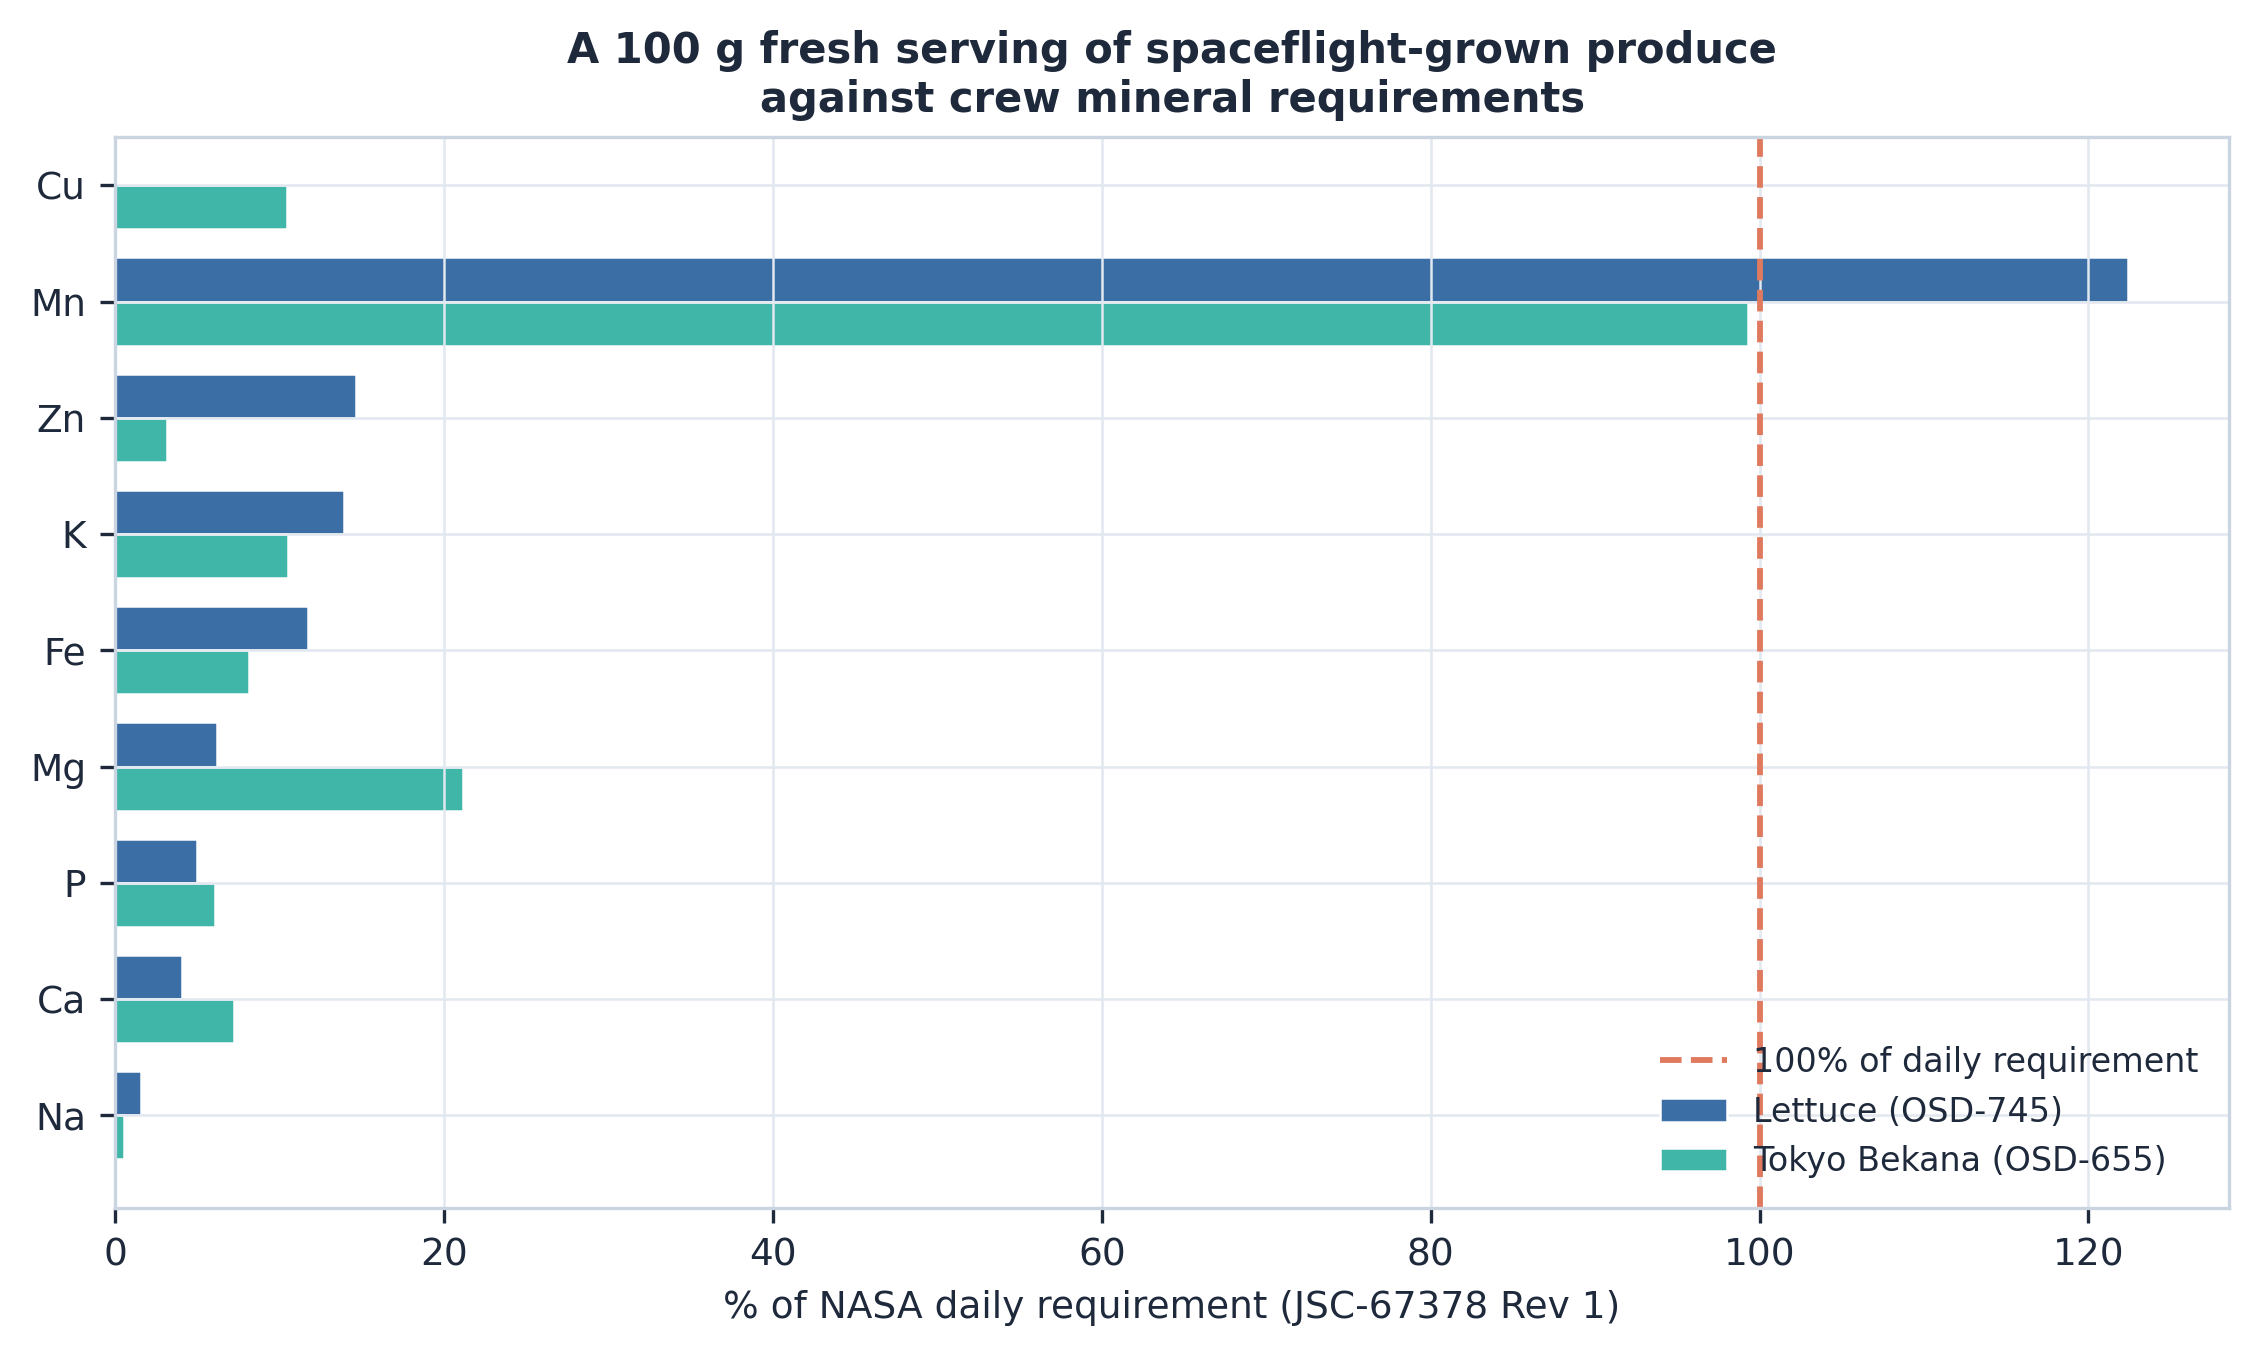
\includegraphics[width=0.88\textwidth]{figures/fig5_serving_contribution.png}
  \caption{Percentage of the NASA daily mineral requirement supplied by a
    100\,g fresh serving of flight-grown produce.}
  \label{fig:serving}
\end{figure}

The overload question can now be answered directly. Reaching NASA's iron upper
limit of 8\,mg/d would require \OverloadFeLet\,kg of fresh lettuce or
\OverloadFeTb\,kg of Tokyo Bekana per day; the zinc limit of 40\,mg/d would
require \OverloadZnLet\,kg and \OverloadZnTb\,kg respectively. A VEG-04A pillow
produced roughly \BiomassFlight\,g fresh, so the iron limit alone would demand
the entire yield of more than twenty pillows daily. Dietary mineral overload
from Veggie produce is not achievable at any plausible harvest scale.

\subsection{Supply-normalised uptake}

Per-pillow water delivery and harvest mass were recovered for \SupplyMatched{}
of \SupplyTotal{} Tokyo Bekana samples (VEG-04A only). Flight pillows received
less water than ground controls (\WaterFlight{} versus \WaterGround\,mL) while
producing comparable biomass (\BiomassFlight{} versus \BiomassGround\,g),
giving a higher apparent water-use efficiency in flight
(\WueFlight{} versus \WueGround\,g fresh mass per litre). Because no dry-matter
fraction is archived, absolute uptake efficiency cannot be computed; the
implications are taken up in Section~\ref{sec:discussion}.
